\documentclass[10pt,xcolor=pdflatex]{beamer}
\usepackage{newcent}
\usepackage[utf8]{inputenc}
%\usepackage[czech]{babel}
\usepackage{hyperref}
\usepackage{fancyvrb}
\usetheme{FIT}

%%%%%%%%%%%%%%%%%%%%%%%%%%%%%%%%%%%%%%%%%%%%%%%%%%%%%%%%%%%%%%%%%%
\title[Reversing malware]{Reverse Engineering of Malware}

\author[]{Matej Kašťák}

\institute[]{Brno University of Technology, Faculty of Information Technology\\
Bo\v{z}et\v{e}chova 1/2. 612 66 Brno - Kr\'alovo Pole\\
login@fit.vutbr.cz}

\date{April 10, 2021}

%%%%%%%%%%%%%%%%%%%%%%%%%%%%%%%%%%%%%%%%%%%%%%%%%%%%%%%%%%%%%%%%%%

\begin{document}

\frame[plain]{\titlepage}

\begin{frame}\frametitle{Agenda \& Goals}

    \begin{itemize}

        \item Introduce \emph{reverse engineering} and basic concepts

        \hfill

        \item \emph{Showcase} tools used for reverse engineering

        \hfill

        \item Use the tools on a real malware sample (Demo)
        
    \end{itemize}
    
\end{frame}


\begin{frame}\frametitle{What is reverse engineering?}

  \begin{columns}
    \column{0.5\textwidth}
    \begin{itemize}
        \item Analyze foreign unknown files
        \item Extract \emph{signatures} that can be used for blocking malware
        \item Gain knowledge how to better \emph{protect} ourselves
    \end{itemize}
    \column{0.5\textwidth}
    \begin{figure}
      \centering
      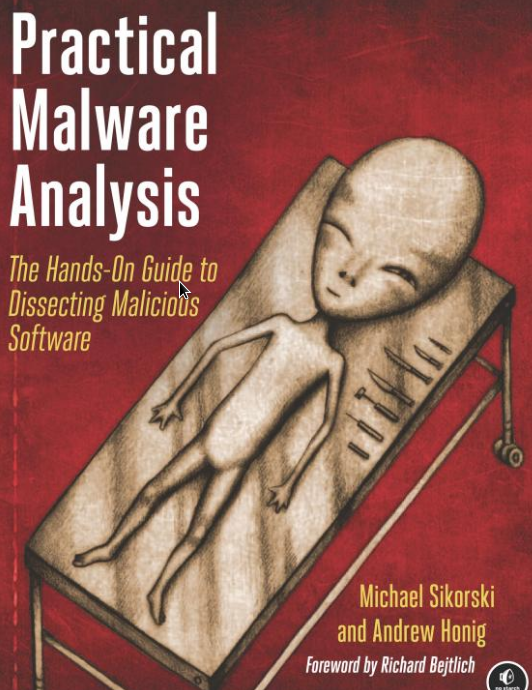
\includegraphics[width=.8\textwidth]{../images/pma.png}
      \caption{Practical Malware Analysis}
    \end{figure}
  \end{columns}

\end{frame}


\begin{frame}\frametitle{Start with the right tools}

  \begin{columns}
    \column{0.5\textwidth}
    \begin{figure}
      \centering
      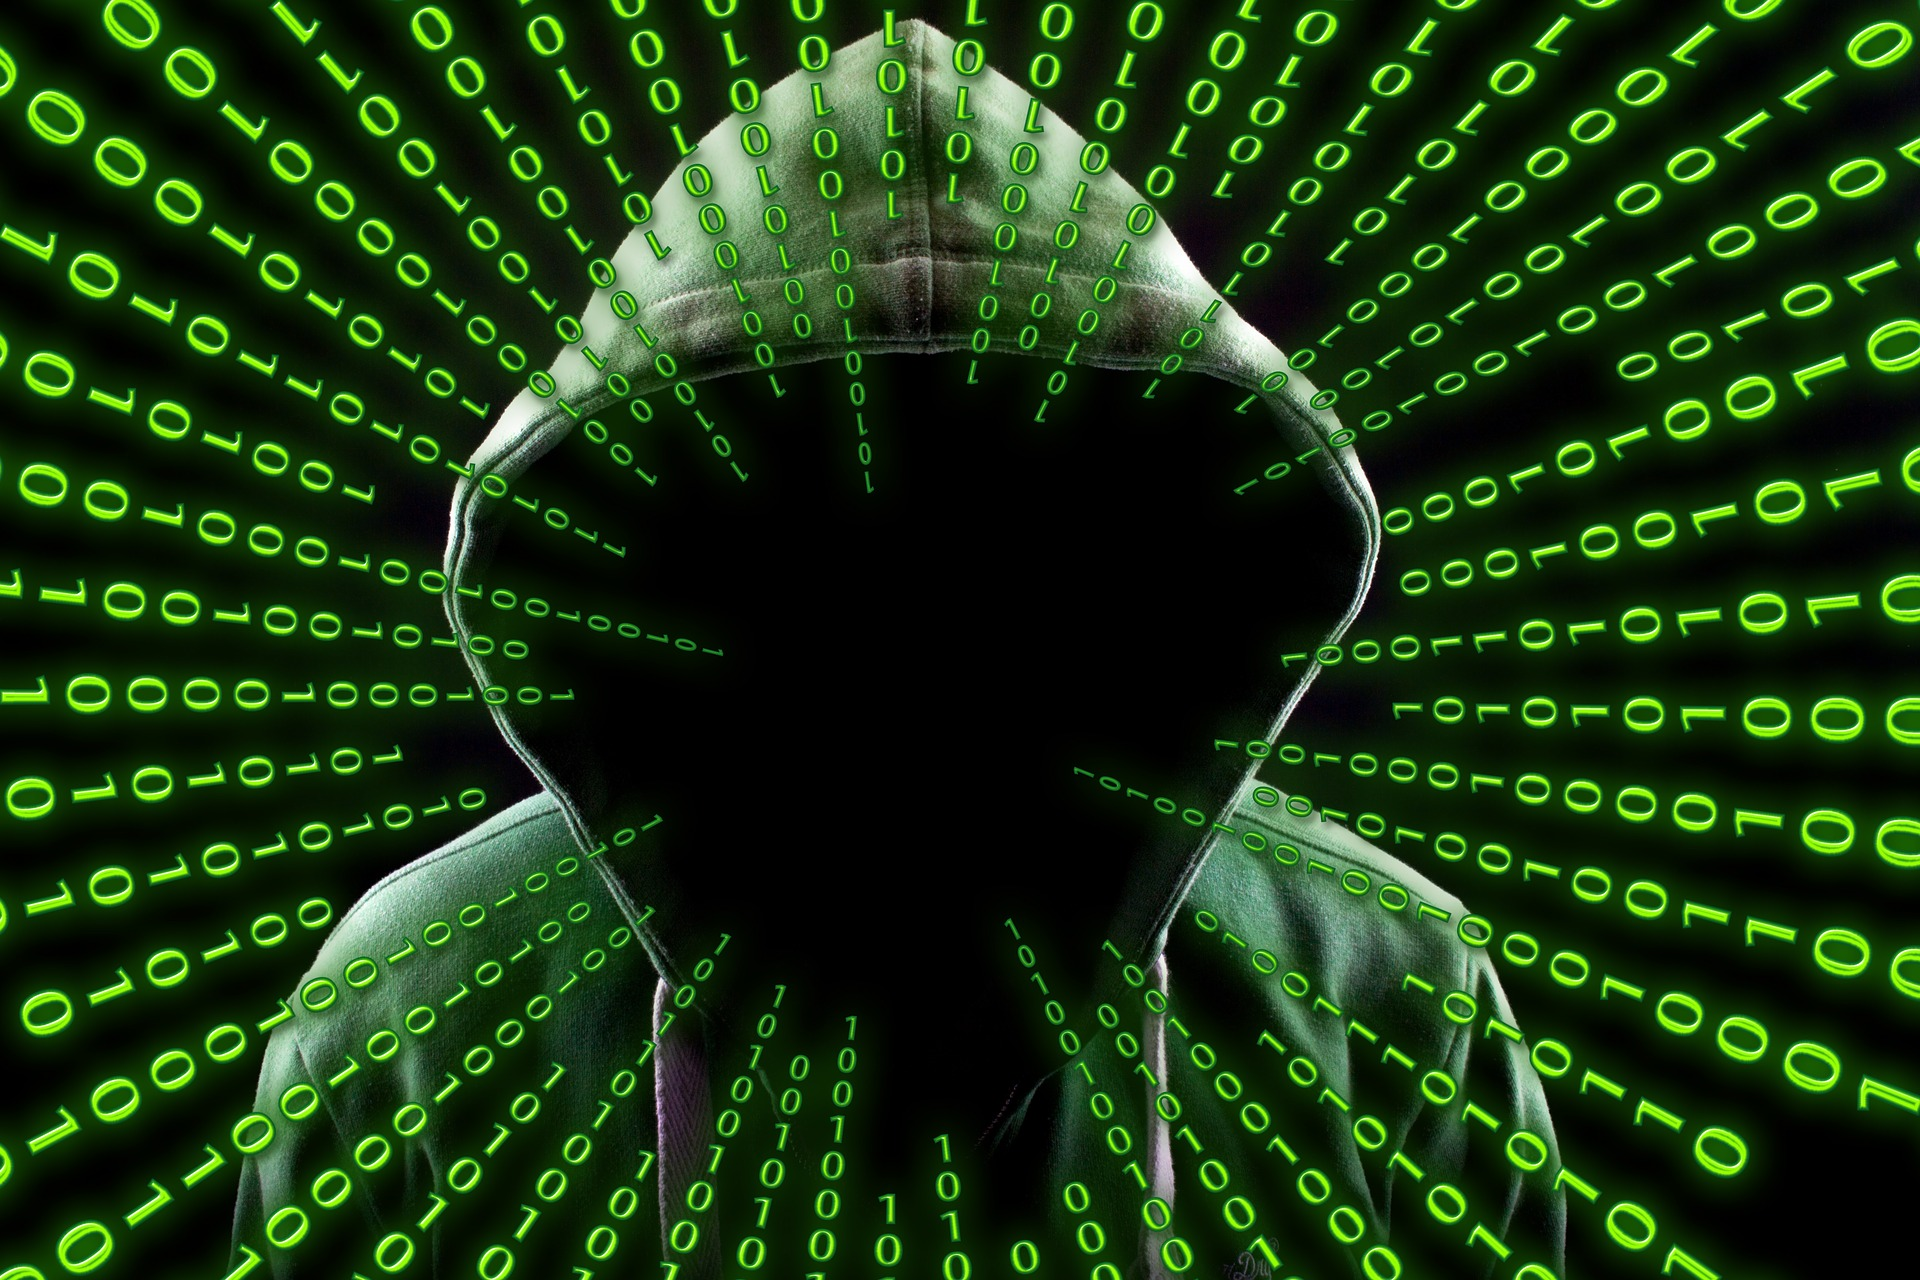
\includegraphics[width=.8\textwidth]{../images/hacker.jpg}
    \caption{Common depiction of a hacker :)}
    \end{figure}
    \column{0.5\textwidth}
    \begin{itemize}
        \item Specialized and complex tools
        \hfill
        \item Require good \emph{low level} understanding of systems
        \hfill
        \item Many of the tools are \emph{really really} expensive
    \end{itemize}
  \end{columns}

\end{frame}


\begin{frame}\frametitle{Static analysis}

  \begin{columns}
    \column{0.4\textwidth}
    \begin{figure}
      \centering
      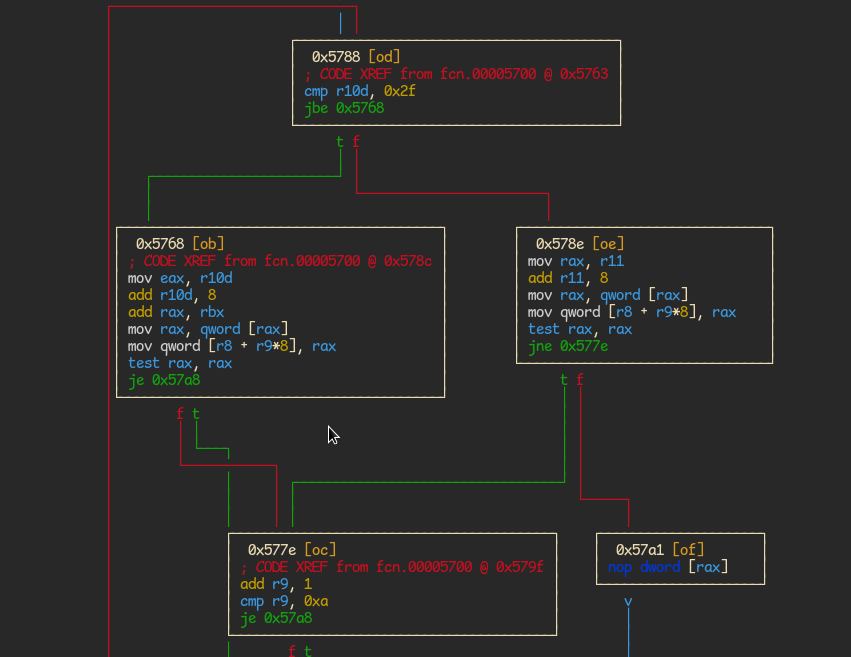
\includegraphics[width=.8\textwidth]{../images/radare2.png}
      \caption{Radare2 example}
    \end{figure}
    \column{0.6\textwidth}
    \begin{itemize}
        \item Disassemblers
            \begin{itemize}
                \item r2/rizin cutter
                \item embedded in other tools
            \end{itemize}
        \item Decompilers
            \begin{itemize}
                \item \emph{IDA}
                \item Ghidra
                \item RetDec
            \end{itemize}
        \item Misc
            \begin{itemize}
                \item strings
                \item entropy
                \item file analyzers
            \end{itemize}
    \end{itemize}
  \end{columns}

\end{frame}

\begin{frame}\frametitle{Ghidra}

    \begin{figure}
      \centering
      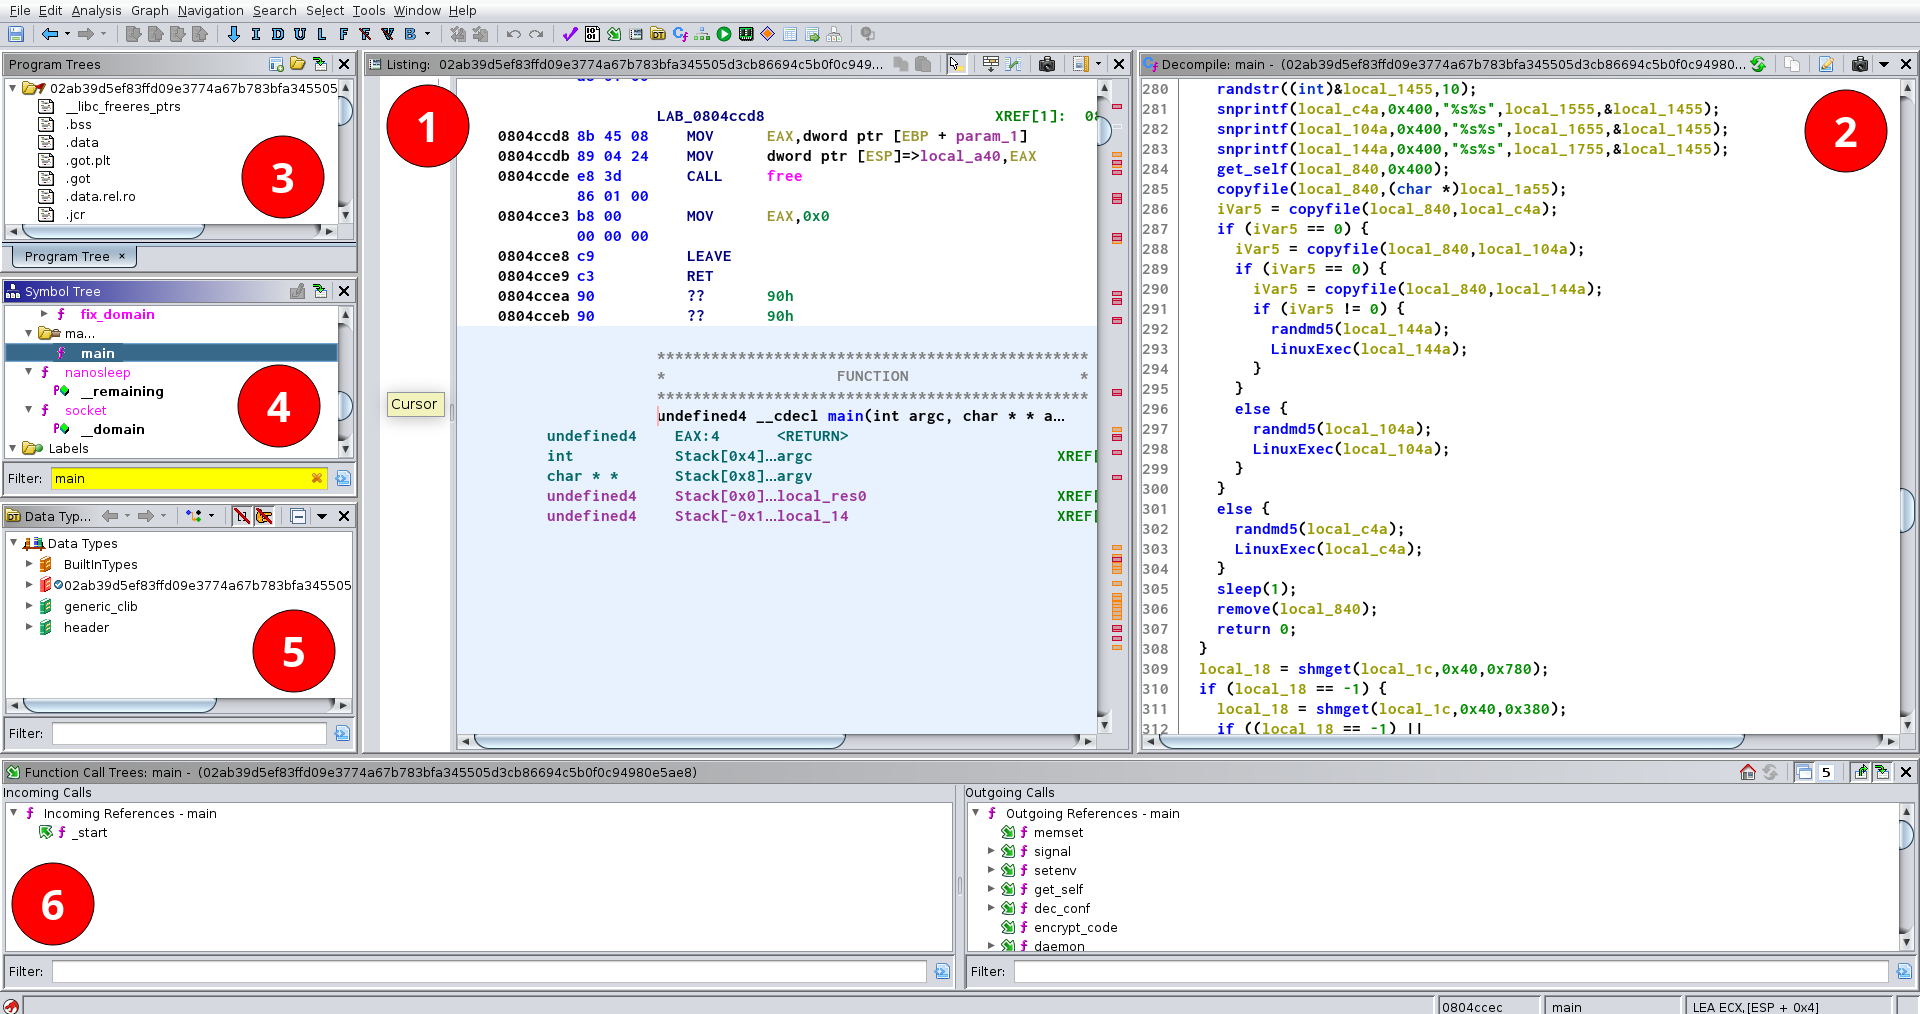
\includegraphics[width=.8\textwidth]{../images/ghidra.png}
      \caption{Ghidra user's interface.}
    \end{figure}
    \begin{itemize}
        \item Open source competitor to IDA pro
        \item Sometimes lacking functionality
    \end{itemize}

\end{frame}


\begin{frame}\frametitle{Dynamic analysis}

  \begin{columns}
    \column{0.5\textwidth}
    \begin{itemize}
        \item Debuggers
            \begin{itemize}

                \item WinDbg / OlyDbg

                \item GDB (stace, ltrace)
                
            \end{itemize}
        \hfill
        \item Sandboxes
            \begin{itemize}

                \item Cuckoo

            \end{itemize}
        \hfill
        \item Symbolic execution
            \begin{itemize}

                \item Angr

            \end{itemize}
    \end{itemize}
    \column{0.5\textwidth}
    \begin{figure}
      \centering
      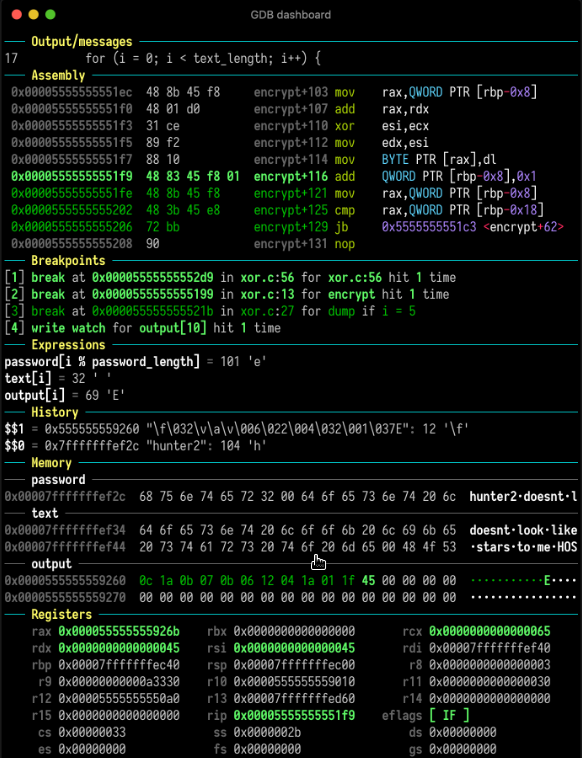
\includegraphics[width=.8\textwidth]{../images/gdb.png}
      \caption{Example GDB output. \tiny Taken from \url{https://github.com/cyrus-and/gdb-dashboard}}
    \end{figure}
  \end{columns}

\end{frame}


\begin{frame}\frametitle{Cuckoo reports}

    \begin{figure}
      \centering
      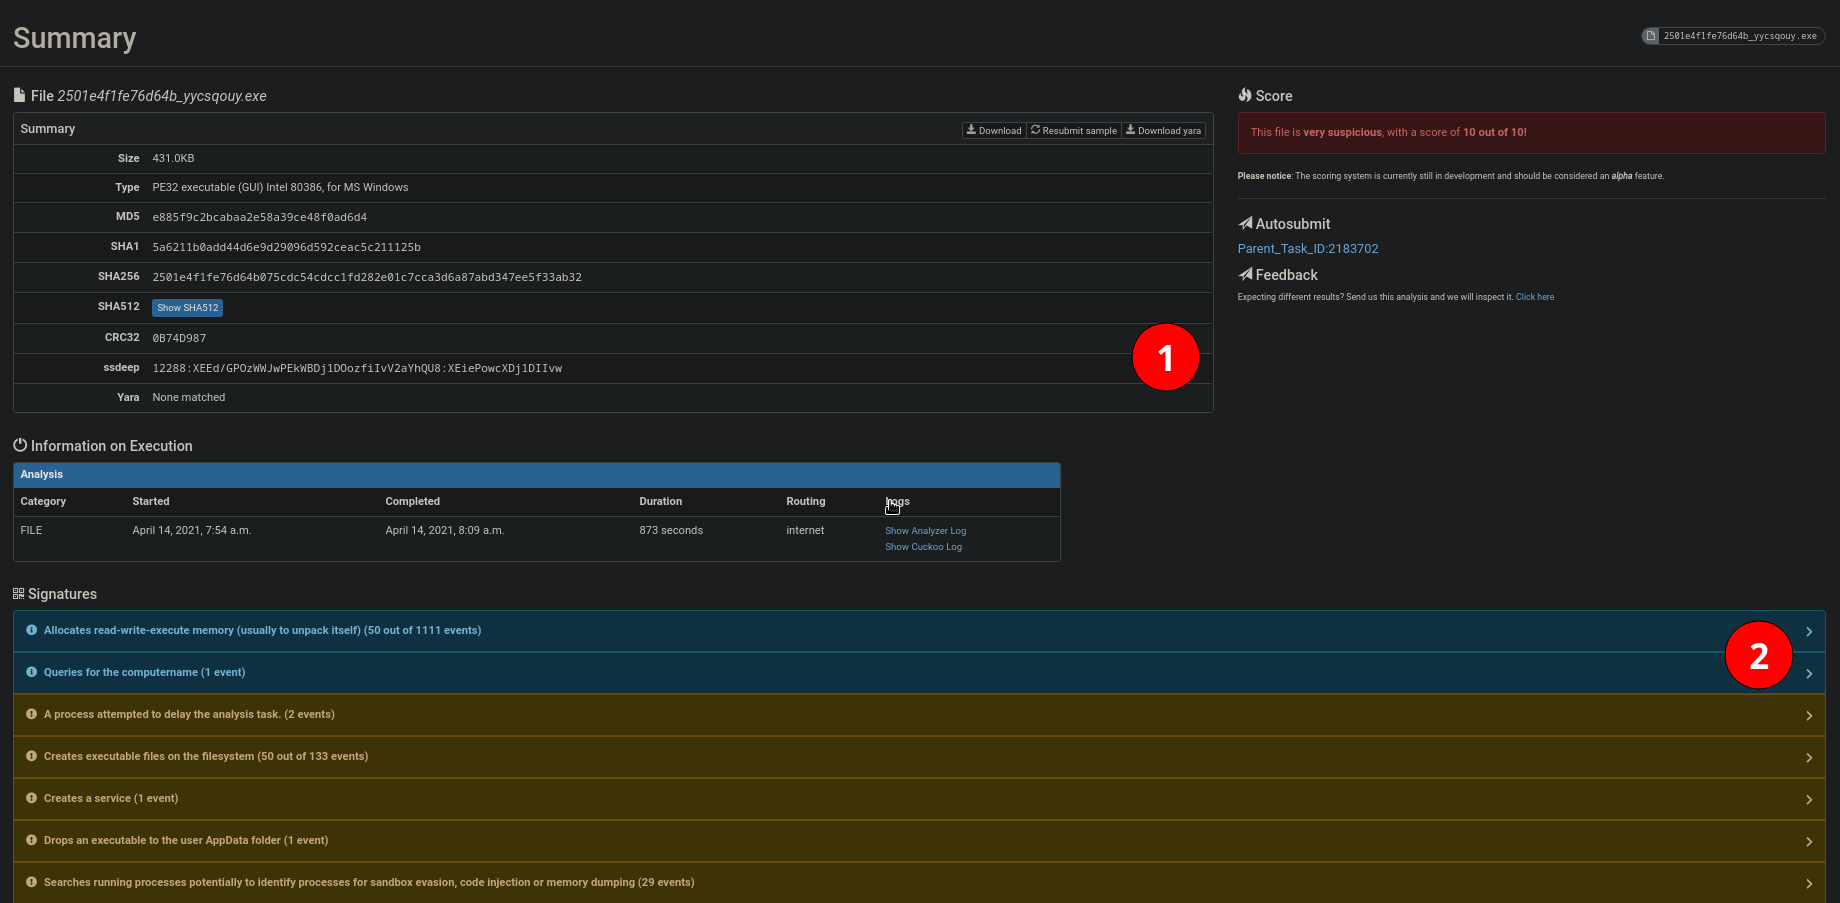
\includegraphics[width=.8\textwidth]{../images/cuckoo.png}
      \caption{Example cuckoo analysis. \tiny Taken from \url{https://cuckoo.cert.ee/}}
    \end{figure}

\end{frame}

\begin{frame}\frametitle{Packers}

  \begin{columns}
    \column{0.5\textwidth}
    \begin{figure}
      \centering
      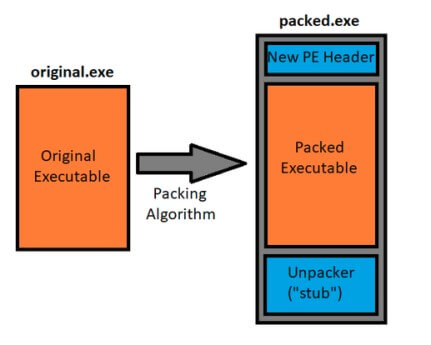
\includegraphics[width=.8\textwidth]{../images/packer.jpg}
    \caption{Packing diagram. \tiny Taken from \url{https://www.arridae.com/blogs/Packed-Malware.php}}
    \end{figure}
    \column{0.5\textwidth}
    \begin{itemize}
        \item Goal is to \emph{avoid detection}
        \hfill
        \item Original binary is embedded into a new one
        \hfill
        \item New binary decodes and executes the original code
        \hfill
        \item Examples
            \begin{itemize}

                \item UPX
                \item Armadillo
                
            \end{itemize}
    \end{itemize}
  \end{columns}

\end{frame}

\bluepage{Demo}

\begin{frame}\frametitle{Summary}
    \begin{itemize}

        \item \emph{Introduced} basic concepts and tools used for reverse engineering

        \hfill

        \item \emph{Analyzed} a malware sample using Ghidra

        \hfill

        \item \emph{Created} program that is able to reverse the encryption schema
        
    \end{itemize}
\end{frame}

\end{document}
